%!TEX root = ../dissertation.tex
\chapter{General Introduction}
\label{introduction}

\newthought{We are currently experiencing a mass extinction event} that parallels
other episodes in earth's history with high rates of biodiversity
decline \citep{Pimm1995, Dirzo2003, Schipper2008, Barnosky2011,
Dirzo2014}. Other than the five previous major extinction events
\citep{Kolbert2014}, it is anthropogenic in origin \citep{Leakey1996,
Ceballos2015} and is associated with global warming \citep{Cook2016,
Wuebbles2017}, large-scale deforestation \citep{Wright2005}, destruction
of marine and freshwater habitats \citep{Burkhead2012}, and introduction
of invasive species \citep{Mooney2001}, all hallmarks of human
influence. Put shortly, the rate at which species go extinct is alarming
\citep{Newbold2016, Ceballos2017, Hallmann2017}, and our children will
likely experience a world with less than half the biodiversity we know
today. While this issue has raised the attention of country leaders and
conservation policies are being put in place worldwide
\citep{Puntaru2017}, this might not be enough to reverse the trend
without sustaining irreparable damage to the ecosystems of the planet.
To make matters worse, there are signs that the issue, despite its
urgency, is fading from public awareness \citep{Kusmanoff2017}. 

Conservation efforts require intimate knowledge of the systems they aim
to preserve: Of course, we cannot save what we do not know. The road
towards understanding the biology and the interaction of species is,
however, travelled on multiple levels. It is not enough to observe the
behaviour or the feeding preferences of an animal to understand the
impact of it being removed from its habitat. It is also not enough to
describe functional morphology to gain insight on ecological
implications. Neither is it sufficient to analyze the genes and draw
conclusions based on their composition and structure. Profound
understanding of any system can only be gained by studying it from
multiple angles and with interdisciplinary approaches. One such approach
is to sequence and analyze the genome of a species: the ``source code of
life'' that defines, by a manifold of means, its appearance, features,
behaviour and interactions with the environment.

The genome, that is, the entirety of DNA of an organism is a composition
of different functional complexes. It does not only contain genes, which
are transcribed to messenger RNA and translated into the proteins that
make up cells and, ultimately, all organisms; in fact, the human gene
repertoire of around 23,000 genes makes up only around \p{2} of the human
genome \citep{Makalowski2001} (Figure \ref{fig:human-genome}). More
prominent components of the human genome include introns (non-coding
sections of genes, around \p{26}), but by far the most voluminous chunk
consists of repetitive elements: DNA segments that occur in sometimes
many copies throughout the genome.  More than half of the three billion
base pairs (Gbp) of the human genome (\p{52}) is occupied by repetitive
elements \citep{Lander2001}. The major part of these repetitive elements
in the human genome, also called repeats, is formed by transposable
elements (\p{45} of the genome).

\begin{figure}
	\centering
  \begin{minipage}[c]{0.3\textwidth}
		\caption[Composition of the human genome]{Composition of the human
		genome. Almost half of the three billion base pairs in the genome is
		attributed to transposable elements of various classes (DNA transposons,
		LTR retrotransposons, LINEs, SINEs). Data source: \citet{Lander2001}}
		\label{fig:human-genome}
  \end{minipage}\hspace{3em}
  \begin{minipage}[c]{0.3\textwidth}
		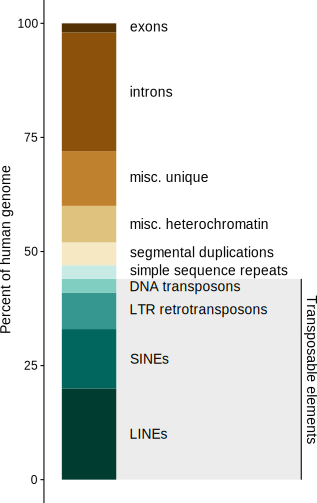
\includegraphics[width=\textwidth]{human}
  \end{minipage}
\end{figure}

Transposable elements (TEs) are also known as ``jumping genes'' or
``parasitic DNA''. They were discovered in the 1940s by their defining
property, the capability of movement within the genome
\citep{McClintock1950}. By duplicating themselves through various
mechanisms that depend on the TE type, TEs can reach copy numbers in the
thousands \citep{Petersen2018} and, like in the human genome (Figure
\ref{fig:human-genome}), be a major contributor to the genome size. This
genome ``inflation'' effect due to TE proliferation has been observed
throughout eukaryotes in general \citep{Chenais2012}, and reiterated in
vertebrates \citep{Chalopin2015}, arthropods \citep{Petersen2018}, and
plants \citep{Staton2015}. 

The genomes of mammals, such as human, and birds exhibit much less
variation in size than, for example, the genomes of arthropods or
amphibians \citep{Gregory2005}. In mammals, genome size varies around
five-fold and in birds even only around two-fold, whereas in insects,
the spread is around 240-fold (Figure \ref{fig:genome-size-spread},
Table \ref{tab:genome-size-spread} on page
\pageref{tab:genome-size-spread}). This immense variation surpasses that
of amphibians, where some species have huge genomes of up to 118 Gbp,
and is paralleled only by the group of bony fishes (Osteichthyes,
excluding lungfishes), which exhibit a genome size spread of around
220-fold. Before the discovery of TEs and non-coding DNA, such as
introns, in the genome, it was assumed that genome size should correlate
with perceived organismic complexity, but the fact that amoeba have
genomes with up to a staggering 670 Gbp \citep{Parfrey2008} did not fit
well with that assumption. This apparent contradiction was named the
``C-value paradox'' and later renamed to ``C-value enigma''
\citep{Gregory2007}, as still a connection between genome size and
organismic complexity appears absent.

\begin{figure}
\centering
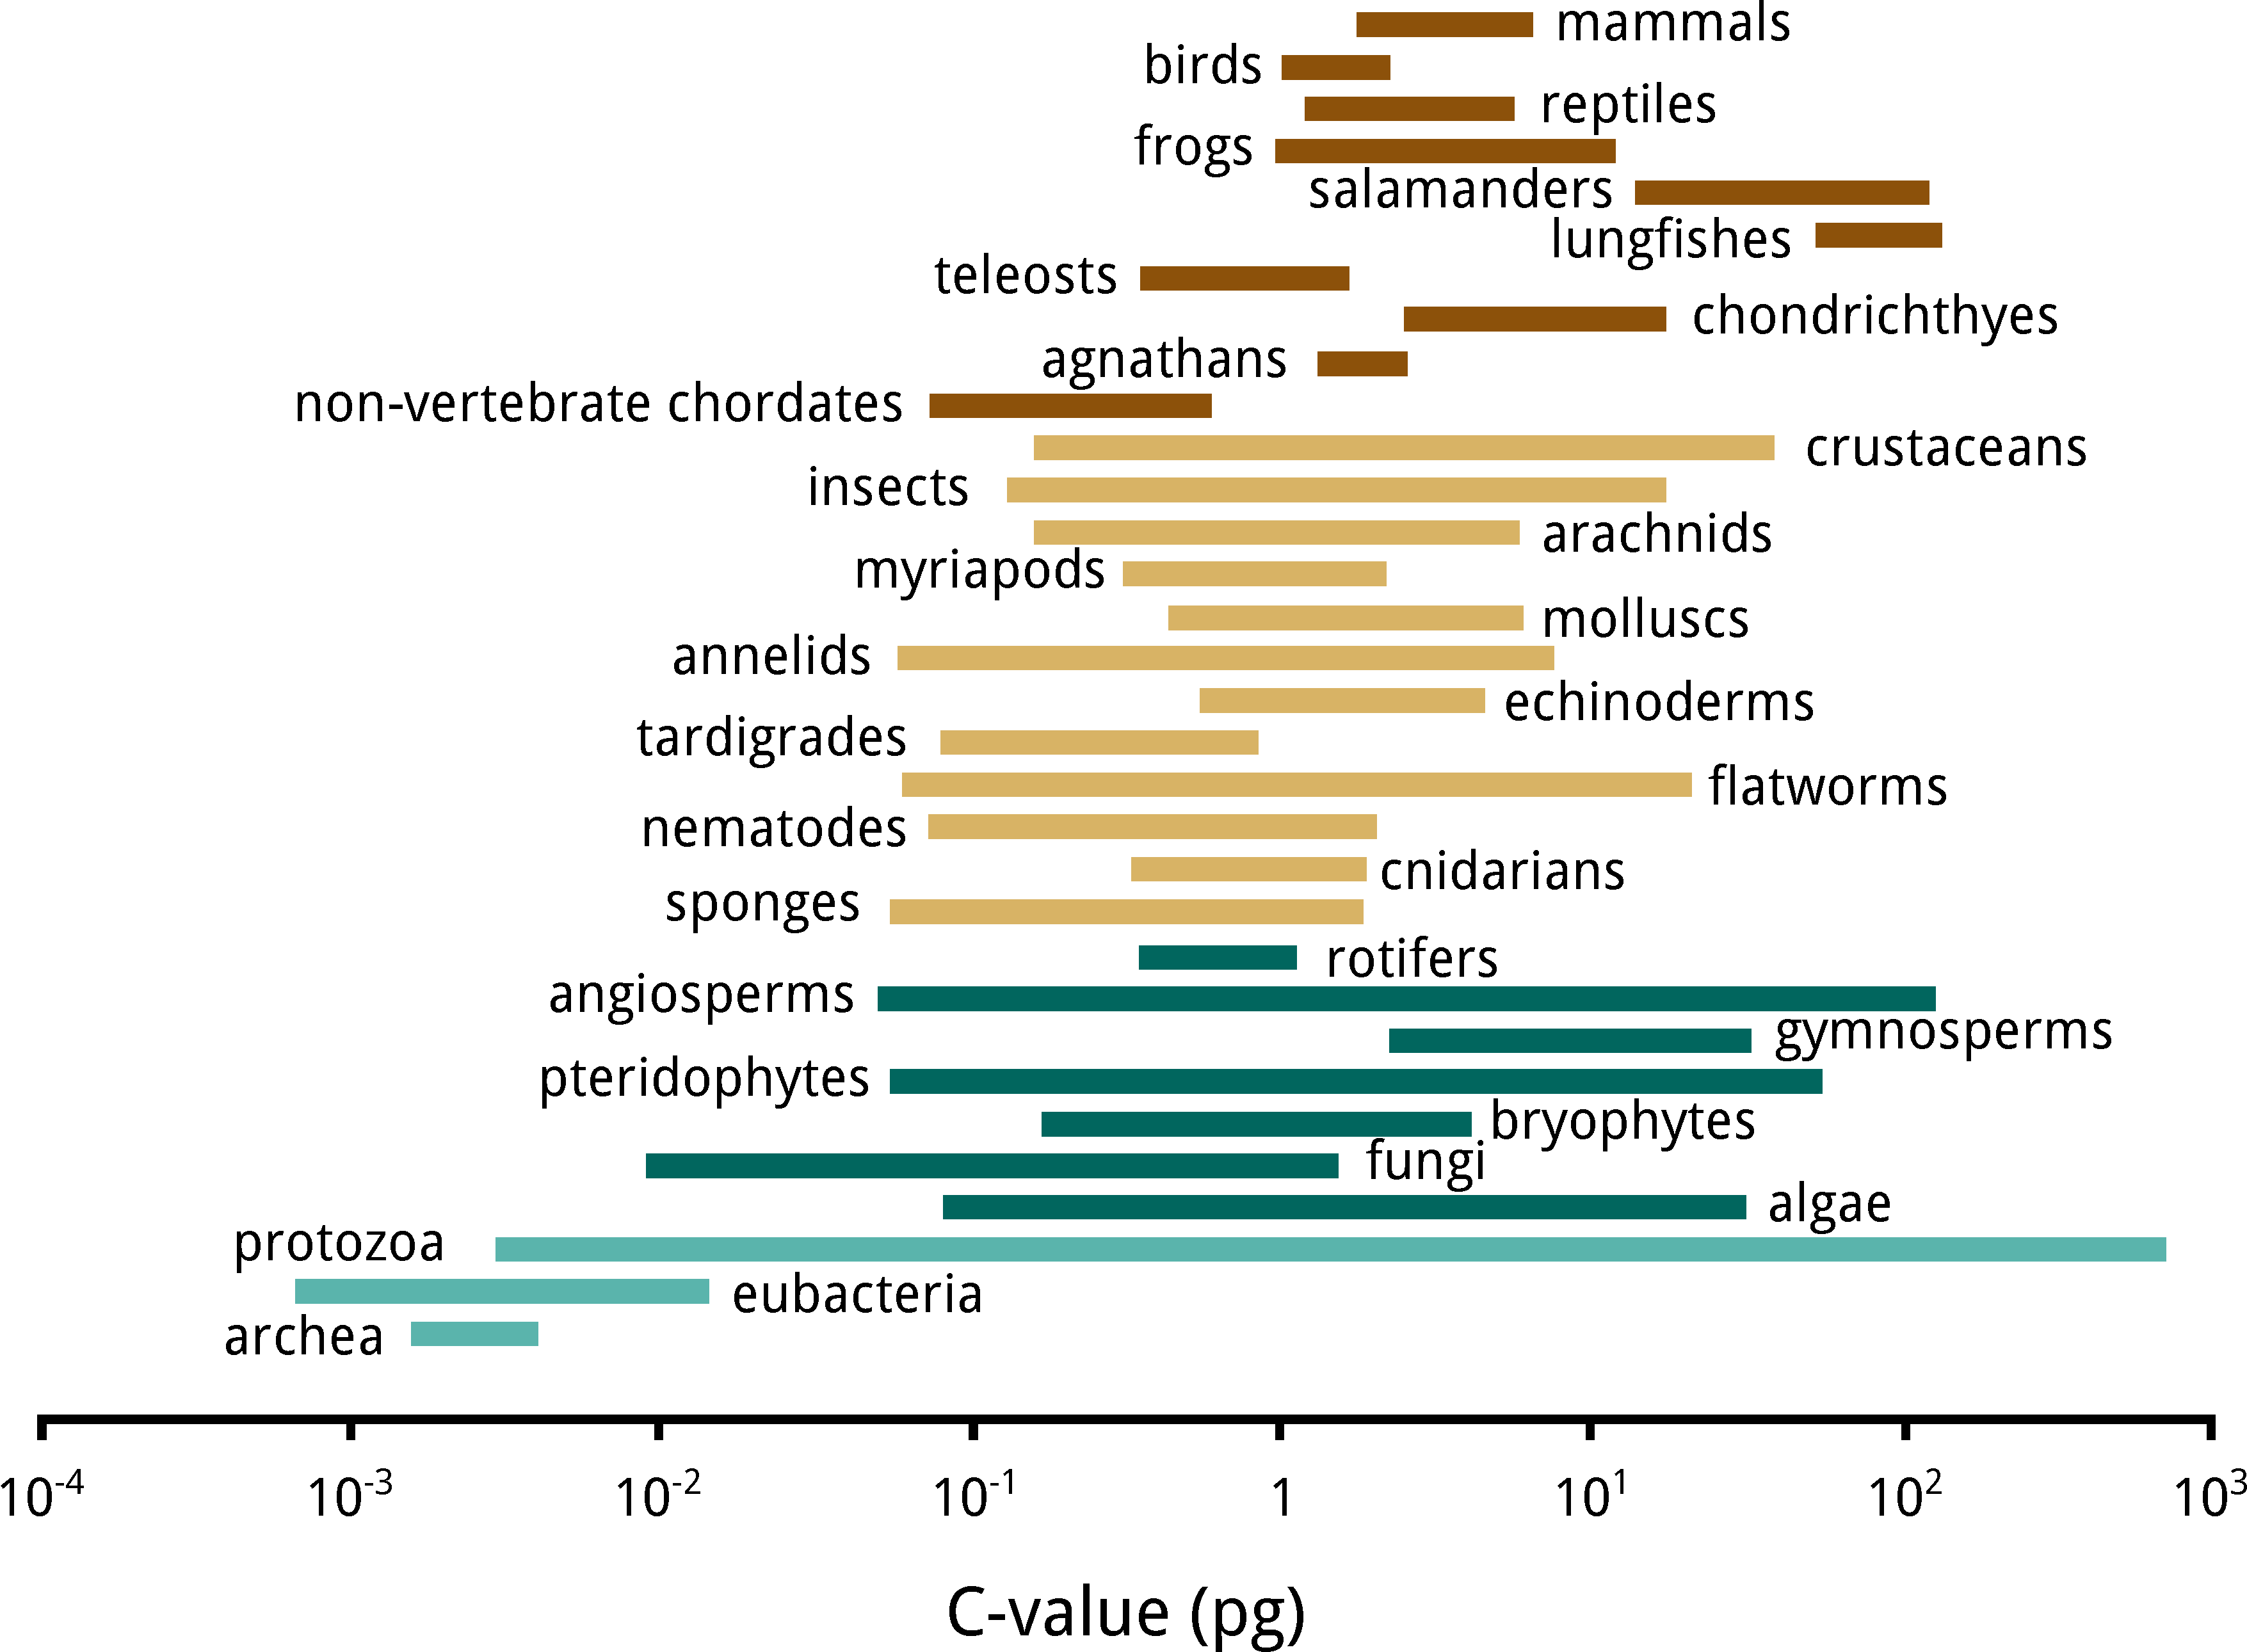
\includegraphics[width=0.7\textwidth]{genome-size-spread}
\caption[Genome size spread in eukaryotes and prokaryotes]{Genome size
spread in eukaryotes and prokaryotes. The C-value is the amount of
haploid nuclear DNA in picogram (pg); one pg DNA is approximately 978
Mbp. Colors are ordered for chordate animals, invertebrate animals,
plants, fungi and algae, and prokaryotes.  Figure modified from
\citet{Gregory2004}.}
\label{fig:genome-size-spread}
\end{figure}

No matter the size, the genome needs to be maintained: repair mechanisms
and transcription machinery as well as error correction use energy. The
transcription and translation error rate increases with genome size
\citep{Zaher2009}, making more repairs necessary. Larger genome size has
been linked to decreased development rate \citep{White2000} and
increased oxygen requirements \citep{Vinogradov1997, Gregory2002}. In
plants \citep{Grime1983}, invertebrates \citep{Gregory2005}, and
vertebrates \citep{Horner1983, Olmo1982, Gregory2000}, it has been shown
that cell size increases with genome size \citep{Dufresne2011}. Larger
cells are also less efficient to maintain and proliferate, and they
divide more slowly \citep{Bennett1977}. In summary, a large genome comes
with a cost. What would be the benefit of having a large genome?

The more genetic material in the genome, the higher the likelihood of
random mutations \citep{Wielgoss2011}. Mutations provide the basis for
genotypic evolution: through natural selection, deleterious changes to
the genome will be removed from populations over time, and beneficial
changes --- or innovations --- prevail. A higher mutation rate is not
always a negative property: it also brings with it a higher rate of
beneficial mutations. Therefore, the genome is thought to reach an
equilibrium between the incurred metabolic cost of sustaining a high
mutation rate (\emph{i.e.}, the damage caused by deleterious mutations),
and the cost of mechanisms that reduce the mutation rate
\citep{Bernstein1987, Altenberg2011}.

The presence and activity of TEs can have disruptive influence on the
genome architecture. By inserting at critical positions, TEs can disable
genes \citep{Kazazian1988}. An insertion in regulatory sequence can
change gene expression \citep{Warnefors2010}. TEs, by way of their
repetitive nature, provide hotspots for ectopic (non-homologous)
recombination \citep{Lim1988, Gray2000, Fiston-Lavier2007}, thus
increasing the likelihood for segmental duplications, deletions, and
inversions \citep{Mathiopoulos1998, Remnant2013}. On the one hand, TEs
are obviously a source of potentially deleterious mutations. On the
other hand, TEs can be ``domesticated'' and genes exapted from TE
sequence \citep{Gahan2001, Daborn2002, Aminetzach2005, Chen2007},
conferring novel functions to the host. Such innovations can happen
within a few hundred generations \citep{Dolgin2006, Struchiner2009,
Kofler2015}. As a famous example, the melanism in the British peppered
moth --- in which camouflage evolved that matches the birch trees
blackened as a result of industrialisation --- is caused by TEs
\citep{Hof2016}. These observations document that TE activity can also
have beneficial effects on the host genome (especially in times of
stress \citep{Chenais2012}), and should therefore not be entirely
subdued.

To keep the TE population in check, defenses that remove or silence TEs
have developed in host organisms. In many groups of organisms, a
multi-layered network of epigenetic regulation mechanisms evolved in
place to prevent TE activity at both the pre- and post-transcriptional
stage. In plants, an epigenetic modification called DNA methylation
prevents TEs from being transcribed and thus from transposing
\citep{Slotkin2007, Lisch2009}. After transcription, proteins from the
RNA interference (RNAi) pathway can disable messenger RNA and thereby
silence TEs \citep{Buchon2006}. Similarly, a class of non-coding RNA,
so-called Piwi-interacting RNA (piRNA) protect the integrity of the
genome, in particular in germline cells, by forming a complex with Piwi
proteins, which can bind and cleave RNA \citep{Zeng2011}. This complex
can recognize and silence target TEs in the RNA stage \citep{Siomi2011, Mondal2018}.
Similar systems were identified in vertebrate genomes \citep{Suzuki2008,
Schubeler2015}; DNA methylation is thought to be a genome defense
mechanism in mammals as well \citep{Yoder1997}. Interestingly,
vertebrate genomes are globally methylated, and in plant genomes, only
gene bodies and TEs are methylated \citep{Suzuki2008}. Fungal genome
exhibit an even more mosaic-like methylation pattern: here, only TEs are
methylated and genes are not. In invertebrates, TEs tend to be
unmethylated; the fruit fly \species{Drosophila melanogaster} does not
even have the methyltransferase enzyme. Likewise, some butterfly species
have lost RNAi pathway genes \citep{Pauli2016}. Thus, these genome
defenses appear to be modular and complementary to one another. They are
effective to a certain extent: permanently inactive TEs become genetic
``cruft'' and are degraded by genetic drift (random mutations over time)
like other parts of the genome that are not subject to selection
\citep{Szitenberg2016}. As a result of these extensive silencing
techniques, it is not surprising that most of the TE population in
extant genomes is inactive \citep{Yoder1997, Zilberman2007}.

There are two major models to explain TE population dynamics in the
genome: the equilibrium model and the burst model \citep{Petrov2011,
Kofler2012, Cridland2013, Blumenstiel2014}. In the equilibrium model,
the TE insertion rate is assumed to be more or less constant, and TEs
are silenced and removed by purifying selection at a likewise constant
rate \citep{Charlesworth1983}. This way, insertion rate and
removal/silencing rate would cancel each other out, and the genome size
remains stable.  The equilibrium model provides a better fit for TE
dynamics under the effects of purifying selection \citep{Barron2014}
than the transposition burst model. The burst model, which is also
termed the non-equilibrium model, predicts that TEs undergo periods of
high transposition activity while otherwise proliferating at a constant
but lower rate. Under the transposition burst model, a positive
correlation between the TE age and frequency would be expected, which
better explains the observed TE age distribution in insect genomes as
well as the large genome size fluctuations during insect evolution,
given that TE abundance is a predictor for genome size
\citep{Alfsnes2017, Petersen2018a}.

Insects are among the most speciose groups of organisms on earth (Figure
\ref{fig:biodiversity} on page \pageref{fig:biodiversity}) and, since
their appearance approximately 480 million years ago (Mya)
\citep{Misof2014}, have conquered land, freshwater, and air (but not
saltwater). Protected by their hard exoskeleton, insect representatives
have invaded virtually all conceivable ecosystems including human
habitations \citep{Bertone2016}.  Insects are immensely diverse in
morphology \citep{Grimaldi2005} and often highly specialized towards a
specific food source, habitat, or lifestyle. Bees, wasps, ants, and
termites, for example, form eusocial communities with a complex caste
system. As disease vectors, mosquitoes are responsible for more human
deaths than all other animals combined \citep{WHO2017, Linnell2011,
Lamarque2009, DeMaddalena2008, Kasturiratne2008, Packer2005}. Beetles,
cicadas, and grasshoppers are examples for an important source of food
for livestock and humans alike as well as a pest with high economic
impact \citep{Oliveira2014}. Obviously, insects play pivotal roles in
most ecosystems of the planet. Insect population diversity and
abundance, however, is declining \citep{Vogel2017} as a result of
widespread human influence (see above), with disastrous reverberations
at all levels of the local food chains.  In order to mount efficient
conservation efforts, a thorough understanding of insect biology is
required.

\begin{figure}
\centering
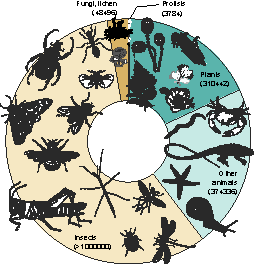
\includegraphics[width=0.75\textwidth]{biodiversity}
\caption[Biodiversity by numbers of species]
{Insects contribute more than half of the currently known species
diversity. Data source: \citet{IUCN2018}}
\label{fig:biodiversity}
\end{figure}

Despite their mega-diversity and ecological importance, insects are
astonishingly understudied on the genomic level compared to other
animals: On 2018-07-06, there were 1,115 published non-insect animal
genome sequences in the NCBI database \citep{OLeary2016} (about \p{0.3}
of the total non-insect species diversity; Figure
\ref{fig:biodiversity}) and 493 insect genomes (\p{0.065}; about five
times less genomes per species).  That number is growing by about 50
genomes per year \citep{OLeary2016}, however at this rate, it will take
more than 150 years to even sequence the genomes of 10 of the insect
biodiversity.  During this time, many species will have gone extinct ---
as it stands, our genome sequencing efforts are losing the race against
man-made biodiversity loss. Ever-improving, massively parallel
sequencing technologies that appeared during the early 2000's
\citep{Behjati2013} have accelerated the pace and accuracy at which
genomes can be sequenced, but it will not be enough. Of many insect
species, we will never be able to obtain the genomic source code, and
this will hamper our understanding of the roles these species occupied
in the interaction network of their habitats.

Comparative genomics studies --- that is, investigations comparing
genomic features of more than one species --- are not only limited by
the fact that for many species, there is no genomic sequence information
available.  Additionally, comparative analyses have to take the
evolutionary history of the species into consideration \citep{Dunn2018},
usually in the form of a phylogenetic tree that conveys information on
the species' relationships. An undisputed phylogenetic tree down to
family level does not exist for insects so far. \citet{Misof2014} and
the 1KITE project \citep{1KITE2018} have inferred a robust backbone
phylogeny for most major insect orders from transcriptomic data (see
below), and several publications have presented order-level phylogenies,
for example for beetles \citep{McKenna2015}, Hymenoptera
\citep{Peters2017, Branstetter2017}, butterflies \citep{Breinholt2018},
and Hemiptera \citep{Johnson2018}. However, accurately reconstructing
species ancestry remains a challenge that has obstructed reliable
comparative analyses in insects so far.

Among the approaches to infer a phylogenetic species tree, the most
informed, because based on matrices with data points numbering in the
millions, is reconstruction from amino acid or nucleotide sequences.
Phylogenetic species tree reconstruction, however, regardless the
method, is no simple task and relies on sophisticated methods on all
stages of the analysis (proposed by \citet{Misof2014}, for example).
Perhaps most of all, selection of the phylogenetic markers (the features
that distinguish species and define their level of relatedness) is
paramount.  Most modern genomic studies use single-copy genes that are
found in all (or almost all) species. The implied assumption is that
these genes share a common ancestry and are related via speciation
events, that is, they are \emph{orthologous} to one another
\citep{Koonin2005} and their phylogeny reflects the species phylogeny.

Several commonly used methods to identify orthologous genes rely on
clustering nucleotide or amino acid sequences based on their similarity
\citep{Chen2007a}. Since orthologs tend to be more similar to each other
than to all other genes in the genomes under comparison
\citep{Altenhoff2012a}, the orthology hypothesis can be tested via a
bi-directional search for similarity applying a best reciprocal hit
(BRH) criterion: Only if the gene in question returns the best hit in
both directions (\ie, the genes are more similar to each other than to
all other genes) it can be assumed to be orthologous. By grouping genes
that share BRH relations, one can form clusters of orthologous genes or
simply orthologous groups (OGs) \citep{Altenhoff2012}. This approach
has been implemented in several software packages for use in genomic
datasets (\eg, \citet{Li2003, Tatusov2003, Berglund2008, Zdobnov2017}).
Obtaining a complete and accurate genome sequence is, however,
associated with technical difficulties and a cost that depends on the
genome size. For these reasons, many phylogenetic studies employ
transcriptomes: the nucleotide sequences of transcripts present in the
sample at the time of RNA fixation \citep{Wang2009}. In contrast to
genomes, however, transcriptomes are inherently incomplete with regard
to the gene set, simply because not all genes are expressed all the time
and may therefore be missing from the sequenced RNA sample. While this
is usually not a problem for phylogenetic analyses \citep{Wiens2006}, it
means that methods to \emph{de novo} infer orthology designed for
genomes cannot not be used on transcriptomic data. To infer orthology
among transcripts, one usually applies a reference-based strategy,
mapping transcripts to known OGs. \citet{Misof2014} used a software that
implements this approach \citep{Ebersberger2009}, however, during the
analyses, it became obvious that it had several design issues that were
non-trivial to fix. Therefore, I concepted and wrote a re-implementation
of the reference-based BRH orthology inference strategy that mitigates
those issues while delivering equal performance \citep{Petersen2017}.
The software, Orthograph (described in chapter \ref{cha:orthograph}),
has been used in several co-authored studies \citep{Mayer2016,
Pauli2016, Bank2017, Dowling2017, Peters2017, Gillung2018, Johnson2018}
that are in the appendix \ref{app:papers-using-orthograph}.

\section{Research questions}

Insects and arthropods in general are unlike vertebrate representatives
on many levels. Like all forms of life, they share general mechanisms of
genetic and genomic functionality and universal elements such as genes
and transposable elements. However, phenotype as well as genome
architecture and dynamics in insects appear drastically different from
vertebrates and plants. Chapter \ref{cha:mobilome} characterizes the
insect TE repertoire in a comparative analysis based on genomic sequence
data from 73 insect and non-insect arthropod species encompassing all
major orders. Differential TE abundance and composition is highlighted
in comparisons between and within insect orders. The correlation between
TE content and genome size in insects is substantiated. Additionally,
the chapter shows that the TE copy age distribution is highly diverse
among insects.

Building on the previous results, chapter \ref{cha:dynamics} presents an
extended analysis on the genomes of 96 arthropod species. 

\section{Roadmap}

Insects are mega-diverse but genomically understudied --- insect
phylogeny on family level mostly unresolved --- 1KITE attempts to change
that --- orthology prediction crucial part of phylogenetic analysis ---
Orthograph identifies orthologs in transcriptomes --- Research questions
--- insect mobilome diversity and evolution --- dynamics of genome size
evolution in insects --- chapter 1: Mobilome --- chapter 2: Genome size
dynamics --- chapter 3: Orthograph --- papers using Orthograph are in
appendix

\begin{table}
\centering\footnotesize
\caption[Genome size spread in Metazoa]{Genome size spread in Metazoa.
Values are in picogram DNA; one pg is approx. 978 mega-basepairs (Mbp).
Data from the Genome Size Database \citep{Gregory2018},
\url{http://www.genomesize.com}, accessed 2018-05-07.}
\label{tab:genome-size-spread}
\begin{tabular}{@{}lllrrrr@{}}
\toprule
Phylum     & Subphylum   & Class          & n    & min  & max   & $\Delta$fold \\
\midrule
Annelida   & --          & Oligochaeta    & 35   & 0.43 & 7.64  & 17.77  \\
Annelida   & --          & Polychaeta     & 100  & 0.06 & 7.2   & 120    \\
Arthropoda & Chelicerata & Arachnida      & 148  & 0.08 & 7.5   & 93.75  \\
Arthropoda & Crustacea   & Branchiopoda   & 68   & 0.16 & 2.91  & 18.19  \\
Arthropoda & Crustacea   & Copepoda       & 73   & 0.14 & 14.68 & 104.86 \\
Arthropoda & Crustacea   & Malacostraca   & 241  & 0.68 & 64.62 & 95.03  \\
Arthropoda & Hexapoda    & Insecta        & 1353 & 0.07 & 16.93 & 241.86 \\
Chordata   & Vertebrata  & Amphibia       & 932  & 0.95 & 120.6 & 126.95 \\
Chordata   & Vertebrata  & Aves           & 903  & 0.91 & 2.16  & 2.37   \\
Chordata   & Vertebrata  & Chondrichthyes & 199  & 1.51 & 17.05 & 11.29  \\
Chordata   & Vertebrata  & Mammalia       & 816  & 1.63 & 8.4   & 5.15   \\
Chordata   & Vertebrata  & Osteichthyes   & 1909 & 0.34 & 74.86 & 220.18 \\
Chordata   & Vertebrata  & Reptilia       & 423  & 1.05 & 5.44  & 5.18   \\
Mollusca   & --          & Bivalvia       & 108  & 0.65 & 5.4   & 8.31   \\
Mollusca   & --          & Gastropoda     & 149  & 0.43 & 7.85  & 18.26  \\
Nematoda   & --          & Secernentea    & 72   & 0.02 & 2.5   & 125    \\
\bottomrule
\end{tabular}
\end{table}
